
\subsection{既存のhikiutilsのコマンド解説}
既存のhikiutilsはコマンド解析ライブラリのoptparseを用いて,コマンドの処理を行っている.
optparseの特徴は,「コマンドの登録,実行method」に分けて記述することが期待されている.
また,CLIの起動の仕方が特徴的である.この二つを取り出して,動作とコードを説明する.

\subsubsection{コマンドの登録と実行メソッド}
\begin{figure}[htbp]\begin{center}
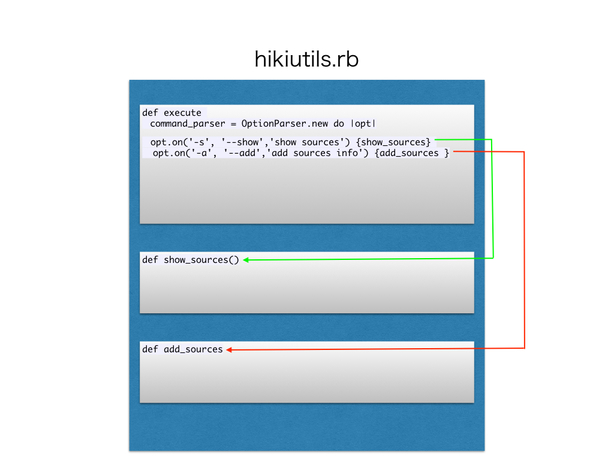
\includegraphics[width=10cm,bb= 0 0 737 553]{../figs/./hikiutils_yamane.005.jpg}
\caption{コマンドの登録と実行メソッドの対応.}
\label{fig:005}
\label{default}\end{center}\end{figure}
optparseでは以下の通り,コマンドの登録と実行が行われる.

\begin{enumerate}
\item OptionParserオブジェクトoptを生成
\item optにコマンドを登録
\item 入力されたコマンドの処理のメソッドへ移動
\end{enumerate}
optparseではOptionParserオブジェクトoptの生成を行い,コマンドをoptに登録することでコマンドを作成することができる.しかし,これはコマンドを登録しているだけでコマンドの一覧ではこれを表示することができるが,コマンドの実行を行うためには実行を行うためのメソッドを作成する必要がある.optparseでのコマンドの実行はoptで登録されたコマンドが入力されることでそれぞれのコマンドの処理を行うメソッドに移動し処理を行う.しかし,このコマンド登録はハイフンを付けたコマンドしか登録ができず,ハイフンなしのコマンド登録はまた別の手段でやらなくてはいけない.
\begin{lstlisting}[style=customRuby,basicstyle={\scriptsize\ttfamily}]
    def execute
      @argv << '--help' if @argv.size==0
      command_parser = OptionParser.new do |opt|
        opt.on('-v', '--version','show program Version.') { |v|
          opt.version = HikiUtils::VERSION
          puts opt.ver
        }
        opt.on('-s', '--show','show sources') {show_sources}
        opt.on('-a', '--add','add sources info') {add_sources }
        opt.on('-t', '--target VAL','set target id') {|val| set_target(val)}
        opt.on('-e', '--edit FILE','open file') {|file| edit_file(file) }

        ...省略...

      end
      begin
        command_parser.parse!(@argv)
      rescue=> eval
        p eval
      end
      dump_sources
      exit
    end    
    
    def show_sources()
      printf("target_no:%i\n",@src[:target])
      printf("editor_command:%s\n",@src[:editor_command])

      ...省略...

    end

    以下略

\end{lstlisting}
\subsubsection{CLIの実行プロセス}
\begin{figure}[htbp]\begin{center}
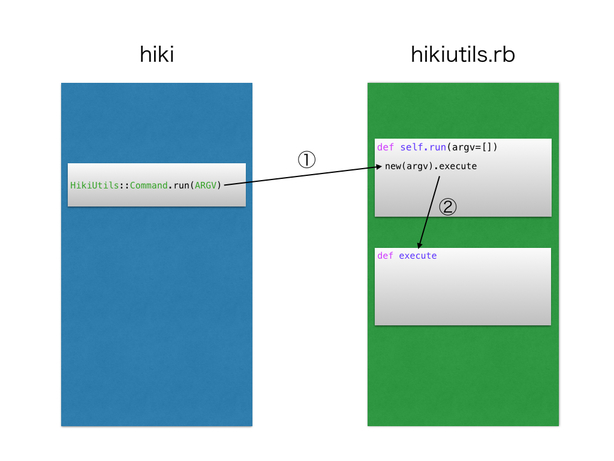
\includegraphics[width=10cm,bb= 0 0 737 553]{../figs/./hikiutils_yamane.007.jpg}
\caption{CLIの実行プロセス.}
\label{fig:007}
\label{default}\end{center}\end{figure}
optparseを用いた場合のCLIの実行プロセスは次の通りとなる.

\begin{enumerate}
\item HikiのHikiUtils::Command.run(ARGV)でhikiutils.rbのrunメソッドを呼ぶ
\item new(argv).executeでexecuteメソッドが実行される
\end{enumerate}
optparseではHikiutils::Command.run(ARGV)を実行される.requireで呼び出されたhikiutils.rbでrunメソッドが実行される.そこでコマンドを登録しているexecuteメソッドへ移動し入力したコマンドと対応させる.そして,対応したコマンドの処理が行われるメソッドに移動することで実行される.このようにoptparseでは実行を行うためのメソッドが必要であるが,

\subsubsection{コード}
optparseの呼び出し側のexe/hikiのコードは次の通りである.
\begin{lstlisting}[style=customRuby,basicstyle={\scriptsize\ttfamily}]
#!/usr/bin/env ruby                                                             

require "hikiutils"

HikiUtils::Command.run(ARGV)
\end{lstlisting}
また呼び出される側のlib/hikiutils.rbのrunおよびexecute部のコードは次の通りとなる.
\begin{lstlisting}[style=customRuby,basicstyle={\scriptsize\ttfamily}]
    def self.run(argv=[])
      print "hikiutils: provide utilities for helping hiki editing.\n"
      new(argv).execute
    end

    def execute
      @argv << '--help' if @argv.size==0
      command_parser = OptionParser.new do |opt|
        opt.on('-v', '--version','show program Version.') { |v|
          opt.version = HikiUtils::VERSION
          puts opt.ver
        }
        opt.on('-s', '--show','show sources') {show_sources}
        opt.on('-a', '--add','add sources info') {add_sources }
        opt.on('-t', '--target VAL','set target id') {|val| set_target(val) }
        opt.on('-e', '--edit FILE','open file') {|file| edit_file(file) }
        opt.on('-l', '--list [FILE]','list files') {|file| list_files(file) }
        opt.on('-u', '--update FILE','update file') {|file| update_file(file) }
        opt.on('-r', '--rsync','rsync files') {rsync_files}
        opt.on('--database FILE','read database file') {|file| db_file(file)}
        opt.on('--display FILE','display converted hikifile') {|file| display(f\
ile)}
        opt.on('-c', '--checkdb','check database file') {check_db}
        opt.on('--remove FILE','remove file') {|file| remove_file(file)}
        opt.on('--move FILES','move file1,file2',Array) {|files| move_file(file\
s)}
        opt.on('--euc FILE','translate file to euc') {|file| euc_file(file) }
        opt.on('--initialize','initialize source directory') {dir_init() }
      end
      begin
        command_parser.parse!(@argv)
      rescue=> eval
        p eval
      end
      dump_sources
      exit
    end  
\end{lstlisting}
